\documentclass{report}

%\usepackage{polski}
\usepackage[utf8]{inputenc}
\usepackage[T1]{fontenc}

\usepackage{graphicx}
\usepackage{caption}
\usepackage{subcaption}
\usepackage{psfrag}
\graphicspath{{./images/}}

\usepackage{amsmath}
\usepackage{amsfonts}

\usepackage{supertabular}
\usepackage{array}
\usepackage{tabularx}
\usepackage{hhline}

\usepackage{hyperref}

\title{A dynamic knowledge \\ management system \\
  \small System efektywnego \\ zarzadzania wiedza}
\author{Cezary Dynak}
%\supervisor{}


\begin{document}
\bibliographystyle{plabbrv}

\maketitle
%\dedication{6cm}{To wife and son}

\tableofcontents

\chapter{Introduction}

Since primary school I was fascinated by structure of knowledge and process of
learning. I started to collect all my notebooks, but there was not much outcome
beside some random notes. I was thinking about creating knowledge management
system for my engineering project, but I choose something else. I tried to make
it my master thesis, but I failed. Finally I just started to making my efforts
public, dreaming that some day I could make PhD out of that. \\

The basic minimalistic idea is just to describe and compare currently existing,
popular knowledge management systems and update it each year.

\chapter{Literature review}
\label{chapter:literature-review}
\section{Goals of the project}
The goal of this project is to create knowledge management system that could
be used in universities to manage academic courses. \cite{web:esco-api}

\begin{figure}[htbp]
  \centering
    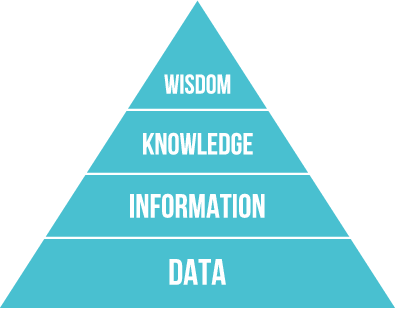
\includegraphics[width=0.5\textwidth]{dikw-pyramid.png}
  \caption{DIKW pyramid}
  \label{fig:panel-dotykowy}
\end{figure}

\section{Qualification frames}

\subsection{Students perspective}
Students are not obligated to knew anything about KRK. Each course is described
in standard way, but its up to each department if it would be presented in a
useful way. As an example, Department of Cybernetics and Robotics hosts on
their webpage compilation of courses description for M.S. program in Embedded
Robotics\cite{web:aer-krk}. Pieces of structured information are also available
from Wroclaw University of Technology web applications, but they are used
mostly for courses sign up:
\paragraph{edukacja.pwr.wroc.pl} -
Students use this portal to sign up to courses. Courses catalog is available
there.
\paragraph{jsos.pwr.edu.pl} -
Students use this portal to accept grades and download week plan. There exist
course search engine, but it only provides courses codes and dates.
\paragraph{akz.pwr.edu.pl} -
Actual Sign up Catalog serves information about sport, language and
humanistic courses. It's also used for sign up purposes.


\subsection{Faculty perspective}
Faculty website is official place for hosting courses description. For now
each faculty serves only documentation in PDF files, like for example Faculty
of Electronics (weka.pwr.edu.pl). There is no system to manage versions of
those documents, they are created in Microsoft Office formats and shared
between staff by email.

\subsection{University perspective}

Rules for qualification frames at university lever are settled by Rector
directives (pol. zarzadzenia Rektora). All directives are available for public
from WRUT website in form of PDF documents, but there is no dedicated website
for qualification frames. Therefore there exists some lower level initiatives
to put this rules in one place, like on Faculty of Electricity website
\cite{web:weny-krk}. There are two main Rector directives that organize
qualification frames: from 2012\cite{web:2012-krk} and from
2015\cite{web:2015-krk}.

\subsection{State perspective}
On the state level the most important document is \textit{higher education
law} from 2005 with many further modifications.
\begin{itemize}
  \item http://isip.sejm.gov.pl/DetailsServlet?id=WDU20051641365
    (Ustawa z dnia 27 lipca 2005 r. Prawo o szkolnictwie wyzszym)
  \item http://www.oa.uj.edu.pl/KRK/A.Krasniewski\_publikacja.pdf
  \item http://ustawa20.nauka.gov.pl
    ("PKA I KRK do radykalnej zmiany."
    "Obnizyc radykalnie role KRK.")
\end{itemize}

\subsection{European perspective}
\begin{itemize}
  \item European Skills, Competences, Qualifications and Occupations
  \item https://ec.europa.eu/esco/portal/home
  \item https://ec.europa.eu/esco/portal/escopedia
\end{itemize}

\subsection{Global perspective}
\begin{itemize}
  \item https://en.wikipedia.org/wiki/Bertrand\_Russell
  \item https://en.wikipedia.org/wiki/Kurt\_Godel
\end{itemize}

\section{Available systems}

\subsection{brainly}

\url{http://www.wirtualnemedia.pl/artykul/brainly-przejmuje-bask-chce-pomagac-w-nauce-za-pomoca-filmow-wideo}

\subsection{Learn Anything}
\begin{itemize}
    \item \url{https://learn-anything.xyz/learn-anything}
    \item \url{https://learn-anything.xyz/computer-graphics/3d-modelling/blender}
\end{itemize}

\chapter{Methodology}
\chapter{Results}
\chapter{Conclusions}

\addcontentsline{toc}{chapter}{Bibliography}
\bibliography{dynamic-knowledge-management-system}

\listoffigures
\listoftables

\end{document}
